\documentclass[twoside]{book}

% Packages required by doxygen
\usepackage{calc}
\usepackage{doxygen}
\usepackage{graphicx}
\usepackage[utf8]{inputenc}
\usepackage{makeidx}
\usepackage{multicol}
\usepackage{multirow}
\usepackage{textcomp}
\usepackage[table]{xcolor}

% Font selection
\usepackage[T1]{fontenc}
\usepackage{mathptmx}
\usepackage[scaled=.90]{helvet}
\usepackage{courier}
\usepackage{amssymb}
\usepackage{sectsty}
\renewcommand{\familydefault}{\sfdefault}
\allsectionsfont{%
  \fontseries{bc}\selectfont%
  \color{darkgray}%
}
\renewcommand{\DoxyLabelFont}{%
  \fontseries{bc}\selectfont%
  \color{darkgray}%
}

% Page & text layout
\usepackage{geometry}
\geometry{%
  a4paper,%
  top=2.5cm,%
  bottom=2.5cm,%
  left=2.5cm,%
  right=2.5cm%
}
\tolerance=750
\hfuzz=15pt
\hbadness=750
\setlength{\emergencystretch}{15pt}
\setlength{\parindent}{0cm}
\setlength{\parskip}{0.2cm}
\makeatletter
\renewcommand{\paragraph}{%
  \@startsection{paragraph}{4}{0ex}{-1.0ex}{1.0ex}{%
    \normalfont\normalsize\bfseries\SS@parafont%
  }%
}
\renewcommand{\subparagraph}{%
  \@startsection{subparagraph}{5}{0ex}{-1.0ex}{1.0ex}{%
    \normalfont\normalsize\bfseries\SS@subparafont%
  }%
}
\makeatother

% Headers & footers
\usepackage{fancyhdr}
\pagestyle{fancyplain}
\fancyhead[LE]{\fancyplain{}{\bfseries\thepage}}
\fancyhead[CE]{\fancyplain{}{}}
\fancyhead[RE]{\fancyplain{}{\bfseries\leftmark}}
\fancyhead[LO]{\fancyplain{}{\bfseries\rightmark}}
\fancyhead[CO]{\fancyplain{}{}}
\fancyhead[RO]{\fancyplain{}{\bfseries\thepage}}
\fancyfoot[LE]{\fancyplain{}{}}
\fancyfoot[CE]{\fancyplain{}{}}
\fancyfoot[RE]{\fancyplain{}{\bfseries\scriptsize Generated on Sat Apr 23 2016 22\-:49\-:56 for Python to C++ translator by Doxygen }}
\fancyfoot[LO]{\fancyplain{}{\bfseries\scriptsize Generated on Sat Apr 23 2016 22\-:49\-:56 for Python to C++ translator by Doxygen }}
\fancyfoot[CO]{\fancyplain{}{}}
\fancyfoot[RO]{\fancyplain{}{}}
\renewcommand{\footrulewidth}{0.4pt}
\renewcommand{\chaptermark}[1]{%
  \markboth{#1}{}%
}
\renewcommand{\sectionmark}[1]{%
  \markright{\thesection\ #1}%
}

% Indices & bibliography
\usepackage{natbib}
\usepackage[titles]{tocloft}
\setcounter{tocdepth}{3}
\setcounter{secnumdepth}{5}
\makeindex

% Hyperlinks (required, but should be loaded last)
\usepackage{ifpdf}
\ifpdf
  \usepackage[pdftex,pagebackref=true]{hyperref}
\else
  \usepackage[ps2pdf,pagebackref=true]{hyperref}
\fi
\hypersetup{%
  colorlinks=true,%
  linkcolor=blue,%
  citecolor=blue,%
  unicode%
}

% Custom commands
\newcommand{\clearemptydoublepage}{%
  \newpage{\pagestyle{empty}\cleardoublepage}%
}


%===== C O N T E N T S =====

\begin{document}

% Titlepage & ToC
\hypersetup{pageanchor=false}
\pagenumbering{roman}
\begin{titlepage}
\vspace*{7cm}
\begin{center}%
{\Large Python to C++ translator }\\
\vspace*{1cm}
{\large Generated by Doxygen 1.8.6}\\
\vspace*{0.5cm}
{\small Sat Apr 23 2016 22:49:56}\\
\end{center}
\end{titlepage}
\clearemptydoublepage
\tableofcontents
\clearemptydoublepage
\pagenumbering{arabic}
\hypersetup{pageanchor=true}

%--- Begin generated contents ---
\chapter{Bug List}
\label{bug}
\hypertarget{bug}{}

\begin{DoxyRefList}
\item[\label{bug__bug000001}%
\hypertarget{bug__bug000001}{}%
File \hyperlink{class__struct_8h}{class\+\_\+struct.h} ]No known bugs.  
\item[\label{bug__bug000003}%
\hypertarget{bug__bug000003}{}%
File \hyperlink{convert__to__cpp_8cpp}{convert\+\_\+to\+\_\+cpp.cpp} ]No known bugs.  
\item[\label{bug__bug000004}%
\hypertarget{bug__bug000004}{}%
File \hyperlink{functionize_8cpp}{functionize.cpp} ]No known bugs.  
\item[\label{bug__bug000005}%
\hypertarget{bug__bug000005}{}%
File \hyperlink{generate__cpp__code_8cpp}{generate\+\_\+cpp\+\_\+code.cpp} ]No known bugs.  
\item[\label{bug__bug000006}%
\hypertarget{bug__bug000006}{}%
File \hyperlink{generated__cpp__classes_8cpp}{generated\+\_\+cpp\+\_\+classes.cpp} ]No known bugs.  
\item[\label{bug__bug000007}%
\hypertarget{bug__bug000007}{}%
File \hyperlink{main_8cpp}{main.cpp} ]No known bugs.  
\item[\label{bug__bug000008}%
\hypertarget{bug__bug000008}{}%
File \hyperlink{render__code_8cpp}{render\+\_\+code.cpp} ]No known bugs.  
\item[\label{bug__bug000002}%
\hypertarget{bug__bug000002}{}%
File \hyperlink{supporting__libs_8h}{supporting\+\_\+libs.h} ]No known bugs. 
\end{DoxyRefList}
\chapter{Module Index}
\section{Modules}
Here is a list of all modules\-:\begin{DoxyCompactList}
\item \contentsline{section}{source\-\_\-code}{\pageref{group__class}}{}
\end{DoxyCompactList}

\chapter{Hierarchical Index}
\section{Class Hierarchy}
This inheritance list is sorted roughly, but not completely, alphabetically\+:\begin{DoxyCompactList}
\item \contentsline{section}{class\+\_\+declaration}{\pageref{structclass__declaration}}{}
\item \contentsline{section}{function\+\_\+declaration}{\pageref{structfunction__declaration}}{}
\item \contentsline{section}{source\+\_\+code}{\pageref{classsource__code}}{}
\item string\begin{DoxyCompactList}
\item \contentsline{section}{artificial\+\_\+string}{\pageref{classartificial__string}}{}
\end{DoxyCompactList}
\end{DoxyCompactList}

\chapter{Class Index}
\section{Class List}
Here are the classes, structs, unions and interfaces with brief descriptions\-:\begin{DoxyCompactList}
\item\contentsline{section}{\hyperlink{classartificial__string}{artificial\-\_\-string} }{\pageref{classartificial__string}}{}
\item\contentsline{section}{\hyperlink{structclass__declaration}{class\-\_\-declaration} }{\pageref{structclass__declaration}}{}
\item\contentsline{section}{\hyperlink{structfunction__declaration}{function\-\_\-declaration} }{\pageref{structfunction__declaration}}{}
\item\contentsline{section}{\hyperlink{classsource__code}{source\-\_\-code} }{\pageref{classsource__code}}{}
\end{DoxyCompactList}

\chapter{File Index}
\section{File List}
Here is a list of all documented files with brief descriptions\+:\begin{DoxyCompactList}
\item\contentsline{section}{Source/\+Header/include/\hyperlink{class__struct_8h}{class\+\_\+struct.\+h} \\*This file defines the structure for storing the classes }{\pageref{class__struct_8h}}{}
\item\contentsline{section}{Source/\+Header/include/\hyperlink{function__struct_8h}{function\+\_\+struct.\+h} }{\pageref{function__struct_8h}}{}
\item\contentsline{section}{Source/\+Header/include/\hyperlink{source__code_8h}{source\+\_\+code.\+h} }{\pageref{source__code_8h}}{}
\item\contentsline{section}{Source/\+Header/supporting\+\_\+libs/\hyperlink{supporting__libs_8h}{supporting\+\_\+libs.\+h} \\*All the string library functions form python translated to cpp }{\pageref{supporting__libs_8h}}{}
\item\contentsline{section}{Source/src/\hyperlink{convert__to__cpp_8cpp}{convert\+\_\+to\+\_\+cpp.\+cpp} \\*This file converts the python code to C++ code in order given to it }{\pageref{convert__to__cpp_8cpp}}{}
\item\contentsline{section}{Source/src/\hyperlink{functionize_8cpp}{functionize.\+cpp} \\*This file sends the python code broken into functions }{\pageref{functionize_8cpp}}{}
\item\contentsline{section}{Source/src/\hyperlink{generate__cpp__code_8cpp}{generate\+\_\+cpp\+\_\+code.\+cpp} \\*This file sends the functions from functionize to \hyperlink{convert__to__cpp_8cpp}{convert\+\_\+to\+\_\+cpp.\+cpp} }{\pageref{generate__cpp__code_8cpp}}{}
\item\contentsline{section}{Source/src/\hyperlink{generated__cpp__classes_8cpp}{generated\+\_\+cpp\+\_\+classes.\+cpp} \\*This function, sends the code to convert to cpp,and keeps in all the details regarding the classes }{\pageref{generated__cpp__classes_8cpp}}{}
\item\contentsline{section}{Source/src/\hyperlink{main_8cpp}{main.\+cpp} \\*Main function to run translator }{\pageref{main_8cpp}}{}
\item\contentsline{section}{Source/src/\hyperlink{render__code_8cpp}{render\+\_\+code.\+cpp} \\*Renders the code in proper format }{\pageref{render__code_8cpp}}{}
\end{DoxyCompactList}

\chapter{Module Documentation}
\hypertarget{group__class}{\section{source\-\_\-code}
\label{group__class}\index{source\-\_\-code@{source\-\_\-code}}
}
This class takes the input file and converts to cpp 
\chapter{Class Documentation}
\hypertarget{classartificial__string}{\section{artificial\-\_\-string Class Reference}
\label{classartificial__string}\index{artificial\-\_\-string@{artificial\-\_\-string}}
}


{\ttfamily \#include $<$supporting\-\_\-libs.\-h$>$}

Inheritance diagram for artificial\-\_\-string\-:\begin{figure}[H]
\begin{center}
\leavevmode
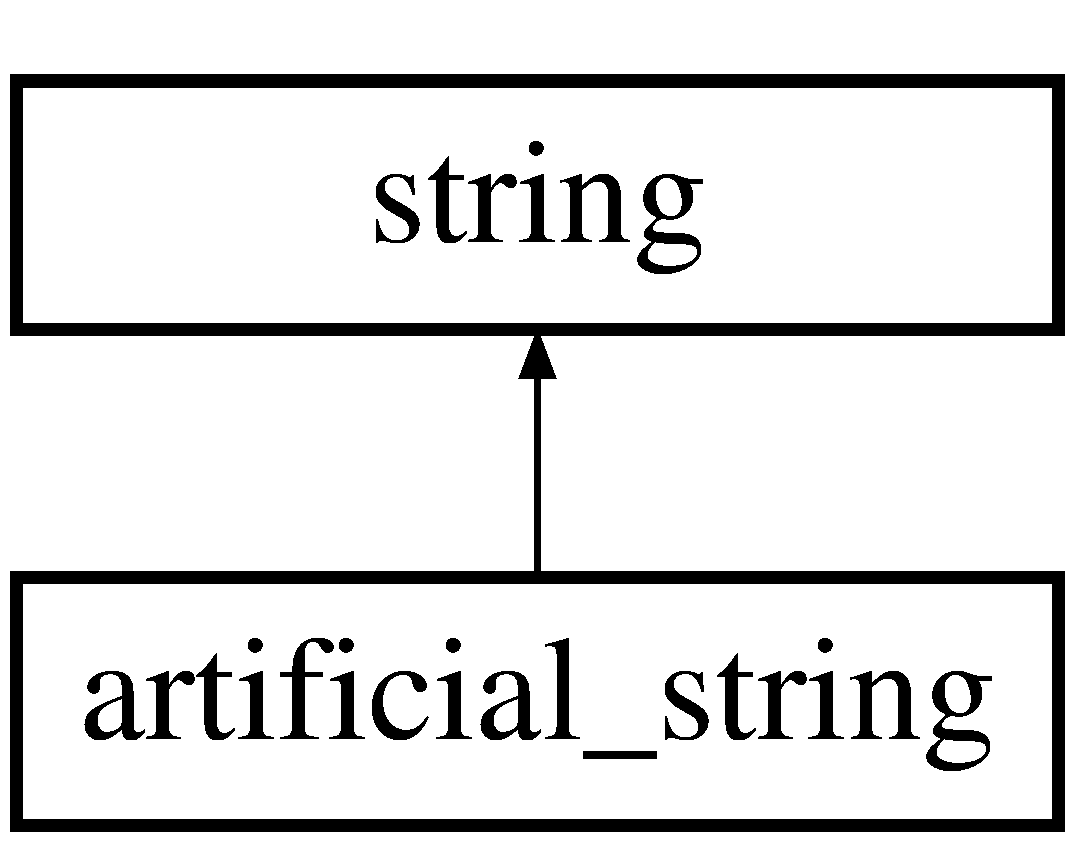
\includegraphics[height=2.000000cm]{classartificial__string}
\end{center}
\end{figure}
\subsection*{Public Member Functions}
\begin{DoxyCompactItemize}
\item 
\hypertarget{classartificial__string_adc63e00c5fc5b22dff3865e89882fa26}{\hyperlink{classartificial__string}{artificial\-\_\-string} {\bfseries operator+} (const \hyperlink{classartificial__string}{artificial\-\_\-string} \&s)}\label{classartificial__string_adc63e00c5fc5b22dff3865e89882fa26}

\item 
\hypertarget{classartificial__string_a059d54e7a346a1c0bafceb3dc34fdc84}{\hyperlink{classartificial__string}{artificial\-\_\-string} {\bfseries operator+} (const std\-::string \&s)}\label{classartificial__string_a059d54e7a346a1c0bafceb3dc34fdc84}

\item 
\hypertarget{classartificial__string_af3c69f5263c568a78f2da48f6f71ec3d}{\hyperlink{classartificial__string}{artificial\-\_\-string} {\bfseries operator+} (const char $\ast$s)}\label{classartificial__string_af3c69f5263c568a78f2da48f6f71ec3d}

\item 
\hypertarget{classartificial__string_a8786c2a3eb31d7543fcc1e512d22562a}{{\bfseries artificial\-\_\-string} (std\-::string s)}\label{classartificial__string_a8786c2a3eb31d7543fcc1e512d22562a}

\item 
\hyperlink{classartificial__string}{artificial\-\_\-string} \hyperlink{classartificial__string_a36c68ec5c9a81edd512bc9e6efe9c80f}{capitalize} ()
\begin{DoxyCompactList}\small\item\em This is a string function to find if the first letter is capital in the artificial string. \end{DoxyCompactList}\item 
int \hyperlink{classartificial__string_a63b0290f444616cb06eb1776af0d80f2}{len} ()
\begin{DoxyCompactList}\small\item\em This is a string function to find the string length of artificial string. \end{DoxyCompactList}\item 
\hyperlink{classartificial__string}{artificial\-\_\-string} \hyperlink{classartificial__string_af6e84a28ddeb314ba6bf36cee3f9f69a}{upper} ()
\begin{DoxyCompactList}\small\item\em This is a string function to convert the artificial string to all capital. \end{DoxyCompactList}\item 
\hyperlink{classartificial__string}{artificial\-\_\-string} \hyperlink{classartificial__string_a62c0582989da7db85168759750892e58}{lower} ()
\begin{DoxyCompactList}\small\item\em This is a string function to convert the artificial string to small letters. \end{DoxyCompactList}\item 
char \hyperlink{classartificial__string_a4cf090a85d3cdcbf8da89720cf0db4e1}{max} ()
\begin{DoxyCompactList}\small\item\em This is a string function to find the alphabetically maximum character in string str. \end{DoxyCompactList}\item 
char \hyperlink{classartificial__string_ab4443974192f4048eb55f3bd2e435885}{min} ()
\begin{DoxyCompactList}\small\item\em This is a string function to find the alphabetically minimum character in string str. \end{DoxyCompactList}\item 
std\-::string \hyperlink{classartificial__string_a4e218591cde8a4ac23dd63c48ca895e3}{swapcase} ()
\begin{DoxyCompactList}\small\item\em This is a string function to swapcase a given string str Basically a capital alphabet converts to small alphabet and a small alphabet to capital. \end{DoxyCompactList}\end{DoxyCompactItemize}
\subsection*{Public Attributes}
\begin{DoxyCompactItemize}
\item 
\hypertarget{classartificial__string_a510a2d4911decf2ee57ae5d95b7ba3d0}{std\-::string {\bfseries str}}\label{classartificial__string_a510a2d4911decf2ee57ae5d95b7ba3d0}

\end{DoxyCompactItemize}
\subsection*{Friends}
\begin{DoxyCompactItemize}
\item 
\hypertarget{classartificial__string_a54896b0297ec3b4f0436a4ac64c9f583}{std\-::ostream \& {\bfseries operator$<$$<$} (std\-::ostream \&output, const \hyperlink{classartificial__string}{artificial\-\_\-string} \&context)}\label{classartificial__string_a54896b0297ec3b4f0436a4ac64c9f583}

\item 
\hypertarget{classartificial__string_a8351339a353e3ef0384266b13d77f789}{std\-::istream \& {\bfseries operator$>$$>$} (std\-::istream \&input, \hyperlink{classartificial__string}{artificial\-\_\-string} \&context)}\label{classartificial__string_a8351339a353e3ef0384266b13d77f789}

\end{DoxyCompactItemize}


\subsection{Detailed Description}
Its not working!! 

\subsection{Member Function Documentation}
\hypertarget{classartificial__string_a36c68ec5c9a81edd512bc9e6efe9c80f}{\index{artificial\-\_\-string@{artificial\-\_\-string}!capitalize@{capitalize}}
\index{capitalize@{capitalize}!artificial_string@{artificial\-\_\-string}}
\subsubsection[{capitalize}]{\setlength{\rightskip}{0pt plus 5cm}{\bf artificial\-\_\-string} artificial\-\_\-string\-::capitalize (
\begin{DoxyParamCaption}
{}
\end{DoxyParamCaption}
)\hspace{0.3cm}{\ttfamily [inline]}}}\label{classartificial__string_a36c68ec5c9a81edd512bc9e6efe9c80f}


This is a string function to find if the first letter is capital in the artificial string. 


\begin{DoxyParams}{Parameters}
{\em Works} & on artificial string str \\
\hline
\end{DoxyParams}
\begin{DoxyReturn}{Returns}
True or False 
\end{DoxyReturn}
\hypertarget{classartificial__string_a63b0290f444616cb06eb1776af0d80f2}{\index{artificial\-\_\-string@{artificial\-\_\-string}!len@{len}}
\index{len@{len}!artificial_string@{artificial\-\_\-string}}
\subsubsection[{len}]{\setlength{\rightskip}{0pt plus 5cm}int artificial\-\_\-string\-::len (
\begin{DoxyParamCaption}
{}
\end{DoxyParamCaption}
)\hspace{0.3cm}{\ttfamily [inline]}}}\label{classartificial__string_a63b0290f444616cb06eb1776af0d80f2}


This is a string function to find the string length of artificial string. 


\begin{DoxyParams}{Parameters}
{\em Works} & on artificial string str \\
\hline
\end{DoxyParams}
\begin{DoxyReturn}{Returns}
size of the artificial string 
\end{DoxyReturn}
\hypertarget{classartificial__string_a62c0582989da7db85168759750892e58}{\index{artificial\-\_\-string@{artificial\-\_\-string}!lower@{lower}}
\index{lower@{lower}!artificial_string@{artificial\-\_\-string}}
\subsubsection[{lower}]{\setlength{\rightskip}{0pt plus 5cm}{\bf artificial\-\_\-string} artificial\-\_\-string\-::lower (
\begin{DoxyParamCaption}
{}
\end{DoxyParamCaption}
)\hspace{0.3cm}{\ttfamily [inline]}}}\label{classartificial__string_a62c0582989da7db85168759750892e58}


This is a string function to convert the artificial string to small letters. 


\begin{DoxyParams}{Parameters}
{\em Works} & on artificial string str \\
\hline
\end{DoxyParams}
\begin{DoxyReturn}{Returns}
string str which is in all small characters 
\end{DoxyReturn}
\hypertarget{classartificial__string_a4cf090a85d3cdcbf8da89720cf0db4e1}{\index{artificial\-\_\-string@{artificial\-\_\-string}!max@{max}}
\index{max@{max}!artificial_string@{artificial\-\_\-string}}
\subsubsection[{max}]{\setlength{\rightskip}{0pt plus 5cm}char artificial\-\_\-string\-::max (
\begin{DoxyParamCaption}
{}
\end{DoxyParamCaption}
)\hspace{0.3cm}{\ttfamily [inline]}}}\label{classartificial__string_a4cf090a85d3cdcbf8da89720cf0db4e1}


This is a string function to find the alphabetically maximum character in string str. 


\begin{DoxyParams}{Parameters}
{\em Works} & on artificial string str \\
\hline
\end{DoxyParams}
\begin{DoxyReturn}{Returns}
maximum alphabetical character in string str 
\end{DoxyReturn}
\hypertarget{classartificial__string_ab4443974192f4048eb55f3bd2e435885}{\index{artificial\-\_\-string@{artificial\-\_\-string}!min@{min}}
\index{min@{min}!artificial_string@{artificial\-\_\-string}}
\subsubsection[{min}]{\setlength{\rightskip}{0pt plus 5cm}char artificial\-\_\-string\-::min (
\begin{DoxyParamCaption}
{}
\end{DoxyParamCaption}
)\hspace{0.3cm}{\ttfamily [inline]}}}\label{classartificial__string_ab4443974192f4048eb55f3bd2e435885}


This is a string function to find the alphabetically minimum character in string str. 


\begin{DoxyParams}{Parameters}
{\em Works} & on artificial string str \\
\hline
\end{DoxyParams}
\begin{DoxyReturn}{Returns}
minimum alphabetical character in string str 
\end{DoxyReturn}
\hypertarget{classartificial__string_a4e218591cde8a4ac23dd63c48ca895e3}{\index{artificial\-\_\-string@{artificial\-\_\-string}!swapcase@{swapcase}}
\index{swapcase@{swapcase}!artificial_string@{artificial\-\_\-string}}
\subsubsection[{swapcase}]{\setlength{\rightskip}{0pt plus 5cm}std\-::string artificial\-\_\-string\-::swapcase (
\begin{DoxyParamCaption}
{}
\end{DoxyParamCaption}
)\hspace{0.3cm}{\ttfamily [inline]}}}\label{classartificial__string_a4e218591cde8a4ac23dd63c48ca895e3}


This is a string function to swapcase a given string str Basically a capital alphabet converts to small alphabet and a small alphabet to capital. 


\begin{DoxyParams}{Parameters}
{\em Works} & on artificial string str \\
\hline
\end{DoxyParams}
\begin{DoxyReturn}{Returns}
a string str in swapped alphabet character 
\end{DoxyReturn}
\hypertarget{classartificial__string_af6e84a28ddeb314ba6bf36cee3f9f69a}{\index{artificial\-\_\-string@{artificial\-\_\-string}!upper@{upper}}
\index{upper@{upper}!artificial_string@{artificial\-\_\-string}}
\subsubsection[{upper}]{\setlength{\rightskip}{0pt plus 5cm}{\bf artificial\-\_\-string} artificial\-\_\-string\-::upper (
\begin{DoxyParamCaption}
{}
\end{DoxyParamCaption}
)\hspace{0.3cm}{\ttfamily [inline]}}}\label{classartificial__string_af6e84a28ddeb314ba6bf36cee3f9f69a}


This is a string function to convert the artificial string to all capital. 


\begin{DoxyParams}{Parameters}
{\em Works} & on artificial string str \\
\hline
\end{DoxyParams}
\begin{DoxyReturn}{Returns}
string str which is in all C\-A\-P\-I\-T\-A\-L 
\end{DoxyReturn}


The documentation for this class was generated from the following file\-:\begin{DoxyCompactItemize}
\item 
Source/\-Header/supporting\-\_\-libs/\hyperlink{supporting__libs_8h}{supporting\-\_\-libs.\-h}\end{DoxyCompactItemize}

\hypertarget{structclass__declaration}{\section{class\-\_\-declaration Struct Reference}
\label{structclass__declaration}\index{class\-\_\-declaration@{class\-\_\-declaration}}
}
\subsection*{Public Attributes}
\begin{DoxyCompactItemize}
\item 
\hypertarget{structclass__declaration_a229b8498e65c3e4507d277e21dc96dd3}{std\-::string {\bfseries name}}\label{structclass__declaration_a229b8498e65c3e4507d277e21dc96dd3}

\item 
\hypertarget{structclass__declaration_ac24e45ec54868aa640b6287779ebe74d}{int {\bfseries num\-\_\-base\-\_\-func}}\label{structclass__declaration_ac24e45ec54868aa640b6287779ebe74d}

\item 
\hypertarget{structclass__declaration_a057735aa678db0370f6c4d24791f78fd}{std\-::vector$<$ std\-::string $>$ {\bfseries base\-\_\-functions}}\label{structclass__declaration_a057735aa678db0370f6c4d24791f78fd}

\end{DoxyCompactItemize}


The documentation for this struct was generated from the following file\-:\begin{DoxyCompactItemize}
\item 
Source/\-Header/include/\hyperlink{class__struct_8h}{class\-\_\-struct.\-h}\end{DoxyCompactItemize}

\hypertarget{structfunction__declaration}{\section{function\-\_\-declaration Struct Reference}
\label{structfunction__declaration}\index{function\-\_\-declaration@{function\-\_\-declaration}}
}
\subsection*{Public Attributes}
\begin{DoxyCompactItemize}
\item 
\hypertarget{structfunction__declaration_a021e9860ca12c3e2835cb21fb4677530}{std\-::string {\bfseries name}}\label{structfunction__declaration_a021e9860ca12c3e2835cb21fb4677530}

\item 
\hypertarget{structfunction__declaration_ae295213d638ea6572a89ccae425476b2}{std\-::string {\bfseries return\-\_\-type}}\label{structfunction__declaration_ae295213d638ea6572a89ccae425476b2}

\item 
\hypertarget{structfunction__declaration_a3e63bb2cf2ed0dd5089fffb8bdee043e}{std\-::vector$<$ string\-\_\-pair $>$ {\bfseries args}}\label{structfunction__declaration_a3e63bb2cf2ed0dd5089fffb8bdee043e}

\end{DoxyCompactItemize}


The documentation for this struct was generated from the following file\-:\begin{DoxyCompactItemize}
\item 
Source/\-Header/include/\hyperlink{function__struct_8h}{function\-\_\-struct.\-h}\end{DoxyCompactItemize}

\hypertarget{classsource__code}{}\section{source\+\_\+code Class Reference}
\label{classsource__code}\index{source\+\_\+code@{source\+\_\+code}}
\subsection*{Public Member Functions}
\begin{DoxyCompactItemize}
\item 
{\bfseries source\+\_\+code} (std\+::string \&st)\hypertarget{classsource__code_abaa948e56e2fcd50d4ce693f724d8687}{}\label{classsource__code_abaa948e56e2fcd50d4ce693f724d8687}

\item 
void \hyperlink{classsource__code_aa728639debb35735e26b6263640af582}{functionize} ()
\begin{DoxyCompactList}\small\item\em Evaluate the python code to break into functions This function takes out the function from python code by undrstanding the length of code that belongs to each function. \end{DoxyCompactList}\item 
void {\bfseries make\+\_\+classes} ()\hypertarget{classsource__code_a3738fc644f820ae38c544b7a07b34141}{}\label{classsource__code_a3738fc644f820ae38c544b7a07b34141}

\item 
void \hyperlink{classsource__code_a2bef035b81554f6bf620603d561af9a7}{generate\+\_\+cpp\+\_\+code} ()
\begin{DoxyCompactList}\small\item\em Sends all functions except main function to \hyperlink{convert__to__cpp_8cpp}{convert\+\_\+to\+\_\+cpp.\+cpp}. \end{DoxyCompactList}\item 
void \hyperlink{classsource__code_a75aeef71dfeb0cdc150e7e4ef9f1cf51}{generate\+\_\+cpp\+\_\+classes} ()
\begin{DoxyCompactList}\small\item\em Sends all classes to convert\+\_\+to\+\_\+cpp\+\_\+classes.\+cpp. \end{DoxyCompactList}\item 
void \hyperlink{classsource__code_a5a9ae302faa54d8e263f1b5c5571f5b1}{render\+\_\+code} ()
\begin{DoxyCompactList}\small\item\em Renders the code in proper format in the output C++ file. \end{DoxyCompactList}\end{DoxyCompactItemize}
\subsection*{Public Attributes}
\begin{DoxyCompactItemize}
\item 
char $\ast$ {\bfseries file\+\_\+name}\hypertarget{classsource__code_a61579010356f4139ec9c2891a16e1687}{}\label{classsource__code_a61579010356f4139ec9c2891a16e1687}

\item 
std\+::vector$<$ line\+\_\+pair $>$ {\bfseries lines}\hypertarget{classsource__code_ab26a720dc9bae50f42103f8b286cf540}{}\label{classsource__code_ab26a720dc9bae50f42103f8b286cf540}

\item 
std\+::vector$<$ int\+\_\+pair $>$ {\bfseries functions}\hypertarget{classsource__code_a75b5ed93456a4bbabf7eaad560630d00}{}\label{classsource__code_a75b5ed93456a4bbabf7eaad560630d00}

\item 
std\+::vector$<$ int\+\_\+pair $>$ {\bfseries classes}\hypertarget{classsource__code_a7fab8b727420c921c947eae6a721b28c}{}\label{classsource__code_a7fab8b727420c921c947eae6a721b28c}

\item 
std\+::vector$<$ std\+::pair$<$ std\+::string, \hyperlink{structfunction__declaration}{function\+\_\+declaration} $>$ $>$ {\bfseries generated\+\_\+cpp\+\_\+code}\hypertarget{classsource__code_ab0191312e5d53f4edf5d9f72d583cc2f}{}\label{classsource__code_ab0191312e5d53f4edf5d9f72d583cc2f}

\item 
std\+::vector$<$ std\+::pair$<$ std\+::string, \hyperlink{structclass__declaration}{class\+\_\+declaration} $>$ $>$ {\bfseries generated\+\_\+cpp\+\_\+classes}\hypertarget{classsource__code_ae3504d0b10056a8876f3023395e0eeba}{}\label{classsource__code_ae3504d0b10056a8876f3023395e0eeba}

\end{DoxyCompactItemize}


\subsection{Member Function Documentation}
\index{source\+\_\+code@{source\+\_\+code}!functionize@{functionize}}
\index{functionize@{functionize}!source\+\_\+code@{source\+\_\+code}}
\subsubsection[{\texorpdfstring{functionize()}{functionize()}}]{\setlength{\rightskip}{0pt plus 5cm}void source\+\_\+code\+::functionize (
\begin{DoxyParamCaption}
{}
\end{DoxyParamCaption}
)}\hypertarget{classsource__code_aa728639debb35735e26b6263640af582}{}\label{classsource__code_aa728639debb35735e26b6263640af582}


Evaluate the python code to break into functions This function takes out the function from python code by undrstanding the length of code that belongs to each function. 


\begin{DoxyParams}{Parameters}
{\em N\+IL} & \\
\hline
\end{DoxyParams}
\begin{DoxyReturn}{Returns}
functions to convert\+\_\+to\+\_\+cpp 
\end{DoxyReturn}
\index{source\+\_\+code@{source\+\_\+code}!generate\+\_\+cpp\+\_\+classes@{generate\+\_\+cpp\+\_\+classes}}
\index{generate\+\_\+cpp\+\_\+classes@{generate\+\_\+cpp\+\_\+classes}!source\+\_\+code@{source\+\_\+code}}
\subsubsection[{\texorpdfstring{generate\+\_\+cpp\+\_\+classes()}{generate_cpp_classes()}}]{\setlength{\rightskip}{0pt plus 5cm}void source\+\_\+code\+::generate\+\_\+cpp\+\_\+classes (
\begin{DoxyParamCaption}
{}
\end{DoxyParamCaption}
)}\hypertarget{classsource__code_a75aeef71dfeb0cdc150e7e4ef9f1cf51}{}\label{classsource__code_a75aeef71dfeb0cdc150e7e4ef9f1cf51}


Sends all classes to convert\+\_\+to\+\_\+cpp\+\_\+classes.\+cpp. 

It takes in the classes from python code and send it convert\+\_\+to\+\_\+cpp\+\_\+classes.\+cpp to make classes in C++. 
\begin{DoxyParams}{Parameters}
{\em N\+IL} & \\
\hline
\end{DoxyParams}
\begin{DoxyReturn}{Returns}
N\+IL 
\end{DoxyReturn}
\index{source\+\_\+code@{source\+\_\+code}!generate\+\_\+cpp\+\_\+code@{generate\+\_\+cpp\+\_\+code}}
\index{generate\+\_\+cpp\+\_\+code@{generate\+\_\+cpp\+\_\+code}!source\+\_\+code@{source\+\_\+code}}
\subsubsection[{\texorpdfstring{generate\+\_\+cpp\+\_\+code()}{generate_cpp_code()}}]{\setlength{\rightskip}{0pt plus 5cm}void source\+\_\+code\+::generate\+\_\+cpp\+\_\+code (
\begin{DoxyParamCaption}
{}
\end{DoxyParamCaption}
)}\hypertarget{classsource__code_a2bef035b81554f6bf620603d561af9a7}{}\label{classsource__code_a2bef035b81554f6bf620603d561af9a7}


Sends all functions except main function to \hyperlink{convert__to__cpp_8cpp}{convert\+\_\+to\+\_\+cpp.\+cpp}. 

It takes in the function form of python code and send it to \hyperlink{convert__to__cpp_8cpp}{convert\+\_\+to\+\_\+cpp.\+cpp} to make functions other than main. 
\begin{DoxyParams}{Parameters}
{\em total} & source code \\
\hline
\end{DoxyParams}
\begin{DoxyReturn}{Returns}
N\+IL 
\end{DoxyReturn}
\index{source\+\_\+code@{source\+\_\+code}!render\+\_\+code@{render\+\_\+code}}
\index{render\+\_\+code@{render\+\_\+code}!source\+\_\+code@{source\+\_\+code}}
\subsubsection[{\texorpdfstring{render\+\_\+code()}{render_code()}}]{\setlength{\rightskip}{0pt plus 5cm}void source\+\_\+code\+::render\+\_\+code (
\begin{DoxyParamCaption}
{}
\end{DoxyParamCaption}
)}\hypertarget{classsource__code_a5a9ae302faa54d8e263f1b5c5571f5b1}{}\label{classsource__code_a5a9ae302faa54d8e263f1b5c5571f5b1}


Renders the code in proper format in the output C++ file. 


\begin{DoxyParams}{Parameters}
{\em N\+IL} & \\
\hline
\end{DoxyParams}
\begin{DoxyReturn}{Returns}
N\+IL 
\end{DoxyReturn}


The documentation for this class was generated from the following files\+:\begin{DoxyCompactItemize}
\item 
Source/\+Header/include/\hyperlink{source__code_8h}{source\+\_\+code.\+h}\item 
Source/src/\hyperlink{functionize_8cpp}{functionize.\+cpp}\item 
Source/src/\hyperlink{generate__cpp__code_8cpp}{generate\+\_\+cpp\+\_\+code.\+cpp}\item 
Source/src/\hyperlink{generated__cpp__classes_8cpp}{generated\+\_\+cpp\+\_\+classes.\+cpp}\item 
Source/src/make\+\_\+classes.\+cpp\item 
Source/src/\hyperlink{render__code_8cpp}{render\+\_\+code.\+cpp}\end{DoxyCompactItemize}

\chapter{File Documentation}
\hypertarget{class__struct_8h}{}\section{Source/\+Header/include/class\+\_\+struct.h File Reference}
\label{class__struct_8h}\index{Source/\+Header/include/class\+\_\+struct.\+h@{Source/\+Header/include/class\+\_\+struct.\+h}}


This file defines the structure for storing the classes.  


\subsection*{Classes}
\begin{DoxyCompactItemize}
\item 
struct \hyperlink{structclass__declaration}{class\+\_\+declaration}
\end{DoxyCompactItemize}


\subsection{Detailed Description}
This file defines the structure for storing the classes. 

\begin{DoxyRefDesc}{Bug}
\item[\hyperlink{bug__bug000001}{Bug}]No known bugs. \end{DoxyRefDesc}

\hypertarget{function__struct_8h}{}\section{Source/\+Header/include/function\+\_\+struct.h File Reference}
\label{function__struct_8h}\index{Source/\+Header/include/function\+\_\+struct.\+h@{Source/\+Header/include/function\+\_\+struct.\+h}}
\subsection*{Classes}
\begin{DoxyCompactItemize}
\item 
struct \hyperlink{structfunction__declaration}{function\+\_\+declaration}
\end{DoxyCompactItemize}
\subsection*{Macros}
\begin{DoxyCompactItemize}
\item 
\#define {\bfseries string\+\_\+pair}~std\+::pair$<$ std\+::string,std\+::string $>$\hypertarget{function__struct_8h_a4890344ede8933ec51bc1fd6e118c5e5}{}\label{function__struct_8h_a4890344ede8933ec51bc1fd6e118c5e5}

\end{DoxyCompactItemize}


\subsection{Detailed Description}
@ brief Structure declaration containing details of functions returned by convert\+\_\+to\+\_\+cpp function 
\hypertarget{source__code_8h}{}\section{Source/\+Header/include/source\+\_\+code.h File Reference}
\label{source__code_8h}\index{Source/\+Header/include/source\+\_\+code.\+h@{Source/\+Header/include/source\+\_\+code.\+h}}
{\ttfamily \#include \char`\"{}class\+\_\+struct.\+h\char`\"{}}\\*
{\ttfamily \#include \char`\"{}function\+\_\+struct.\+h\char`\"{}}\\*
\subsection*{Classes}
\begin{DoxyCompactItemize}
\item 
class \hyperlink{classsource__code}{source\+\_\+code}
\end{DoxyCompactItemize}
\subsection*{Macros}
\begin{DoxyCompactItemize}
\item 
\#define {\bfseries max\+\_\+number\+\_\+of\+\_\+variables}~100\hypertarget{source__code_8h_a00605126c8138510ac4002699665fc6c}{}\label{source__code_8h_a00605126c8138510ac4002699665fc6c}

\item 
\#define {\bfseries tab\+\_\+size}~4\hypertarget{source__code_8h_a345958bec3164ee303d9a5b753af45ab}{}\label{source__code_8h_a345958bec3164ee303d9a5b753af45ab}

\item 
\#define {\bfseries line\+\_\+pair}~std\+::pair$<$std\+::string,int$>$\hypertarget{source__code_8h_af38cd416e1be448ba692d740f7964a68}{}\label{source__code_8h_af38cd416e1be448ba692d740f7964a68}

\item 
\#define {\bfseries int\+\_\+pair}~std\+::pair$<$int,int$>$\hypertarget{source__code_8h_ab062142353dea0e5861291aa8c23c75c}{}\label{source__code_8h_ab062142353dea0e5861291aa8c23c75c}

\end{DoxyCompactItemize}


\subsection{Detailed Description}
brief Class definition 
\hypertarget{supporting__libs_8h}{}\section{Source/\+Header/supporting\+\_\+libs/supporting\+\_\+libs.h File Reference}
\label{supporting__libs_8h}\index{Source/\+Header/supporting\+\_\+libs/supporting\+\_\+libs.\+h@{Source/\+Header/supporting\+\_\+libs/supporting\+\_\+libs.\+h}}


All the string library functions form python translated to cpp.  


{\ttfamily \#include $<$regex$>$}\\*
{\ttfamily \#include $<$vector$>$}\\*
{\ttfamily \#include $<$algorithm$>$}\\*
{\ttfamily \#include $<$string$>$}\\*
{\ttfamily \#include $<$string.\+h$>$}\\*
{\ttfamily \#include $<$iostream$>$}\\*
{\ttfamily \#include $<$fstream$>$}\\*
{\ttfamily \#include $<$stdio.\+h$>$}\\*
{\ttfamily \#include $<$ctype.\+h$>$}\\*
{\ttfamily \#include $<$map$>$}\\*
{\ttfamily \#include $<$stdlib.\+h$>$}\\*
\subsection*{Classes}
\begin{DoxyCompactItemize}
\item 
class \hyperlink{classartificial__string}{artificial\+\_\+string}
\end{DoxyCompactItemize}


\subsection{Detailed Description}
All the string library functions form python translated to cpp. 

\begin{DoxyRefDesc}{Bug}
\item[\hyperlink{bug__bug000002}{Bug}]No known bugs. \end{DoxyRefDesc}

\hypertarget{convert__to__cpp_8cpp}{}\section{Source/src/convert\+\_\+to\+\_\+cpp.cpp File Reference}
\label{convert__to__cpp_8cpp}\index{Source/src/convert\+\_\+to\+\_\+cpp.\+cpp@{Source/src/convert\+\_\+to\+\_\+cpp.\+cpp}}


This file converts the python code to C++ code in order given to it.  


{\ttfamily \#include $<$vector$>$}\\*
{\ttfamily \#include $<$string$>$}\\*
{\ttfamily \#include $<$string.\+h$>$}\\*
{\ttfamily \#include $<$iostream$>$}\\*
{\ttfamily \#include $<$ctype.\+h$>$}\\*
{\ttfamily \#include $<$algorithm$>$}\\*
{\ttfamily \#include $<$map$>$}\\*
{\ttfamily \#include $<$stdlib.\+h$>$}\\*
{\ttfamily \#include $<$sstream$>$}\\*
{\ttfamily \#include \char`\"{}../\+Header/include/function\+\_\+struct.\+h\char`\"{}}\\*
{\ttfamily \#include \char`\"{}../\+Header/include/source\+\_\+code.\+h\char`\"{}}\\*
\subsection*{Functions}
\begin{DoxyCompactItemize}
\item 
std\+::string \hyperlink{convert__to__cpp_8cpp_a21c1bfd8feaefba529e0c220836b29ee}{eval\+\_\+expr} (std\+::string \&s)
\begin{DoxyCompactList}\small\item\em Evaluate the python code to C++ code. \end{DoxyCompactList}\item 
bool \hyperlink{convert__to__cpp_8cpp_ab9dd2b78c85900f6d49a2457c4cb99d0}{is\+\_\+symbol} (char c)
\begin{DoxyCompactList}\small\item\em Checks the special symbols used. \end{DoxyCompactList}\item 
std\+::string \hyperlink{convert__to__cpp_8cpp_ab797c01777c71119ed06da98053d1812}{expr\+\_\+type} (std\+::string \&expr, std\+::map$<$ std\+::string, std\+::string $>$ \&variables)
\begin{DoxyCompactList}\small\item\em Decides the type of the variable. \end{DoxyCompactList}\item 
void \hyperlink{convert__to__cpp_8cpp_a9aad2372701a968f1a9517d6f52c8e12}{break\+\_\+into\+\_\+words} (std\+::string \&line, std\+::vector$<$ std\+::string $>$ \&tokens)
\begin{DoxyCompactList}\small\item\em Breaks the python string to words. \end{DoxyCompactList}\item 
std\+::string \hyperlink{convert__to__cpp_8cpp_a653b093fe6844a0f3111cff6a9f448ea}{map\+\_\+type} (std\+::string s, int l)
\begin{DoxyCompactList}\small\item\em Wraps mentioned type of variable. \end{DoxyCompactList}\item 
std\+::string \hyperlink{convert__to__cpp_8cpp_a2279105a73ae9907985afc9c451d354e}{itoa} (int number)
\begin{DoxyCompactList}\small\item\em Converts the integer into string. \end{DoxyCompactList}\item 
void \hyperlink{convert__to__cpp_8cpp_a6c9b7704837b714c714081745485127d}{convert\+\_\+to\+\_\+cpp} (unsigned long int start, unsigned long int end, std\+::vector$<$ line\+\_\+pair $>$ \&lines, std\+::string \&converted\+\_\+code, \hyperlink{structfunction__declaration}{function\+\_\+declaration} $\ast$\+\_\+function, std\+::map$<$ std\+::string, std\+::string $>$ \&variables)
\begin{DoxyCompactList}\small\item\em Converts Python code to C++ code in order. \end{DoxyCompactList}\end{DoxyCompactItemize}


\subsection{Detailed Description}
This file converts the python code to C++ code in order given to it. 

\begin{DoxyRefDesc}{Bug}
\item[\hyperlink{bug__bug000003}{Bug}]No known bugs. \end{DoxyRefDesc}


\subsection{Function Documentation}
\index{convert\+\_\+to\+\_\+cpp.\+cpp@{convert\+\_\+to\+\_\+cpp.\+cpp}!break\+\_\+into\+\_\+words@{break\+\_\+into\+\_\+words}}
\index{break\+\_\+into\+\_\+words@{break\+\_\+into\+\_\+words}!convert\+\_\+to\+\_\+cpp.\+cpp@{convert\+\_\+to\+\_\+cpp.\+cpp}}
\subsubsection[{\texorpdfstring{break\+\_\+into\+\_\+words(std\+::string \&line, std\+::vector$<$ std\+::string $>$ \&tokens)}{break_into_words(std::string &line, std::vector< std::string > &tokens)}}]{\setlength{\rightskip}{0pt plus 5cm}void break\+\_\+into\+\_\+words (
\begin{DoxyParamCaption}
\item[{std\+::string \&}]{line, }
\item[{std\+::vector$<$ std\+::string $>$ \&}]{tokens}
\end{DoxyParamCaption}
)}\hypertarget{convert__to__cpp_8cpp_a9aad2372701a968f1a9517d6f52c8e12}{}\label{convert__to__cpp_8cpp_a9aad2372701a968f1a9517d6f52c8e12}


Breaks the python string to words. 

It breaks the python string into words and breaks into token 
\begin{DoxyParams}{Parameters}
{\em python} & string \\
\hline
\end{DoxyParams}
\begin{DoxyReturn}{Returns}
N\+IL 
\end{DoxyReturn}
\index{convert\+\_\+to\+\_\+cpp.\+cpp@{convert\+\_\+to\+\_\+cpp.\+cpp}!convert\+\_\+to\+\_\+cpp@{convert\+\_\+to\+\_\+cpp}}
\index{convert\+\_\+to\+\_\+cpp@{convert\+\_\+to\+\_\+cpp}!convert\+\_\+to\+\_\+cpp.\+cpp@{convert\+\_\+to\+\_\+cpp.\+cpp}}
\subsubsection[{\texorpdfstring{convert\+\_\+to\+\_\+cpp(unsigned long int start, unsigned long int end, std\+::vector$<$ line\+\_\+pair $>$ \&lines, std\+::string \&converted\+\_\+code, function\+\_\+declaration $\ast$\+\_\+function, std\+::map$<$ std\+::string, std\+::string $>$ \&variables)}{convert_to_cpp(unsigned long int start, unsigned long int end, std::vector< line_pair > &lines, std::string &converted_code, function_declaration *_function, std::map< std::string, std::string > &variables)}}]{\setlength{\rightskip}{0pt plus 5cm}void convert\+\_\+to\+\_\+cpp (
\begin{DoxyParamCaption}
\item[{unsigned long int}]{start, }
\item[{unsigned long int}]{end, }
\item[{std\+::vector$<$ line\+\_\+pair $>$ \&}]{lines, }
\item[{std\+::string \&}]{converted\+\_\+code, }
\item[{{\bf function\+\_\+declaration} $\ast$}]{\+\_\+function, }
\item[{std\+::map$<$ std\+::string, std\+::string $>$ \&}]{variables}
\end{DoxyParamCaption}
)}\hypertarget{convert__to__cpp_8cpp_a6c9b7704837b714c714081745485127d}{}\label{convert__to__cpp_8cpp_a6c9b7704837b714c714081745485127d}


Converts Python code to C++ code in order. 

It takes lines of code in python and converts it to C++ in exactly the same order from beginning to ending. 
\begin{DoxyParams}{Parameters}
{\em starting} & line, ending line,vector of lines of code, function parameters, variables table \\
\hline
\end{DoxyParams}
\begin{DoxyReturn}{Returns}
N\+IL 
\end{DoxyReturn}
\index{convert\+\_\+to\+\_\+cpp.\+cpp@{convert\+\_\+to\+\_\+cpp.\+cpp}!eval\+\_\+expr@{eval\+\_\+expr}}
\index{eval\+\_\+expr@{eval\+\_\+expr}!convert\+\_\+to\+\_\+cpp.\+cpp@{convert\+\_\+to\+\_\+cpp.\+cpp}}
\subsubsection[{\texorpdfstring{eval\+\_\+expr(std\+::string \&s)}{eval_expr(std::string &s)}}]{\setlength{\rightskip}{0pt plus 5cm}std\+::string eval\+\_\+expr (
\begin{DoxyParamCaption}
\item[{std\+::string \&}]{s}
\end{DoxyParamCaption}
)}\hypertarget{convert__to__cpp_8cpp_a21c1bfd8feaefba529e0c220836b29ee}{}\label{convert__to__cpp_8cpp_a21c1bfd8feaefba529e0c220836b29ee}


Evaluate the python code to C++ code. 


\begin{DoxyParams}{Parameters}
{\em python} & expression \\
\hline
\end{DoxyParams}
\begin{DoxyReturn}{Returns}
converted C++ expression. 
\end{DoxyReturn}
\index{convert\+\_\+to\+\_\+cpp.\+cpp@{convert\+\_\+to\+\_\+cpp.\+cpp}!expr\+\_\+type@{expr\+\_\+type}}
\index{expr\+\_\+type@{expr\+\_\+type}!convert\+\_\+to\+\_\+cpp.\+cpp@{convert\+\_\+to\+\_\+cpp.\+cpp}}
\subsubsection[{\texorpdfstring{expr\+\_\+type(std\+::string \&expr, std\+::map$<$ std\+::string, std\+::string $>$ \&variables)}{expr_type(std::string &expr, std::map< std::string, std::string > &variables)}}]{\setlength{\rightskip}{0pt plus 5cm}std\+::string expr\+\_\+type (
\begin{DoxyParamCaption}
\item[{std\+::string \&}]{expr, }
\item[{std\+::map$<$ std\+::string, std\+::string $>$ \&}]{variables}
\end{DoxyParamCaption}
)}\hypertarget{convert__to__cpp_8cpp_ab797c01777c71119ed06da98053d1812}{}\label{convert__to__cpp_8cpp_ab797c01777c71119ed06da98053d1812}


Decides the type of the variable. 

It checks and decides the type of variables in C++ for corresponding variable in python 
\begin{DoxyParams}{Parameters}
{\em python} & expression \\
\hline
\end{DoxyParams}
\begin{DoxyReturn}{Returns}
C++ type for the variable 
\end{DoxyReturn}
\index{convert\+\_\+to\+\_\+cpp.\+cpp@{convert\+\_\+to\+\_\+cpp.\+cpp}!is\+\_\+symbol@{is\+\_\+symbol}}
\index{is\+\_\+symbol@{is\+\_\+symbol}!convert\+\_\+to\+\_\+cpp.\+cpp@{convert\+\_\+to\+\_\+cpp.\+cpp}}
\subsubsection[{\texorpdfstring{is\+\_\+symbol(char c)}{is_symbol(char c)}}]{\setlength{\rightskip}{0pt plus 5cm}bool is\+\_\+symbol (
\begin{DoxyParamCaption}
\item[{char}]{c}
\end{DoxyParamCaption}
)}\hypertarget{convert__to__cpp_8cpp_ab9dd2b78c85900f6d49a2457c4cb99d0}{}\label{convert__to__cpp_8cpp_ab9dd2b78c85900f6d49a2457c4cb99d0}


Checks the special symbols used. 

It reads the character and checks if it is a special symbol used in python 
\begin{DoxyParams}{Parameters}
{\em character} & c \\
\hline
\end{DoxyParams}
\begin{DoxyReturn}{Returns}
Tells if the read symbol is special or not. 
\end{DoxyReturn}
\index{convert\+\_\+to\+\_\+cpp.\+cpp@{convert\+\_\+to\+\_\+cpp.\+cpp}!itoa@{itoa}}
\index{itoa@{itoa}!convert\+\_\+to\+\_\+cpp.\+cpp@{convert\+\_\+to\+\_\+cpp.\+cpp}}
\subsubsection[{\texorpdfstring{itoa(int number)}{itoa(int number)}}]{\setlength{\rightskip}{0pt plus 5cm}std\+::string itoa (
\begin{DoxyParamCaption}
\item[{int}]{number}
\end{DoxyParamCaption}
)}\hypertarget{convert__to__cpp_8cpp_a2279105a73ae9907985afc9c451d354e}{}\label{convert__to__cpp_8cpp_a2279105a73ae9907985afc9c451d354e}


Converts the integer into string. 

It converts a integer in its corresponding string form 
\begin{DoxyParams}{Parameters}
{\em integer} & number \\
\hline
\end{DoxyParams}
\begin{DoxyReturn}{Returns}
number as string 
\end{DoxyReturn}
\index{convert\+\_\+to\+\_\+cpp.\+cpp@{convert\+\_\+to\+\_\+cpp.\+cpp}!map\+\_\+type@{map\+\_\+type}}
\index{map\+\_\+type@{map\+\_\+type}!convert\+\_\+to\+\_\+cpp.\+cpp@{convert\+\_\+to\+\_\+cpp.\+cpp}}
\subsubsection[{\texorpdfstring{map\+\_\+type(std\+::string s, int l)}{map_type(std::string s, int l)}}]{\setlength{\rightskip}{0pt plus 5cm}std\+::string map\+\_\+type (
\begin{DoxyParamCaption}
\item[{std\+::string}]{s, }
\item[{int}]{l}
\end{DoxyParamCaption}
)}\hypertarget{convert__to__cpp_8cpp_a653b093fe6844a0f3111cff6a9f448ea}{}\label{convert__to__cpp_8cpp_a653b093fe6844a0f3111cff6a9f448ea}


Wraps mentioned type of variable. 

It reads the type if mentioned in the python code 
\begin{DoxyParams}{Parameters}
{\em string} & type that has type ,int l \\
\hline
\end{DoxyParams}
\begin{DoxyReturn}{Returns}
The type of the variable. 
\end{DoxyReturn}

\hypertarget{functionize_8cpp}{}\section{Source/src/functionize.cpp File Reference}
\label{functionize_8cpp}\index{Source/src/functionize.\+cpp@{Source/src/functionize.\+cpp}}


This file sends the python code broken into functions.  


{\ttfamily \#include $<$vector$>$}\\*
{\ttfamily \#include $<$string$>$}\\*
{\ttfamily \#include $<$string.\+h$>$}\\*
{\ttfamily \#include $<$iostream$>$}\\*
{\ttfamily \#include \char`\"{}../\+Header/include/function\+\_\+struct.\+h\char`\"{}}\\*
{\ttfamily \#include \char`\"{}../\+Header/include/source\+\_\+code.\+h\char`\"{}}\\*
\subsection*{Macros}
\begin{DoxyCompactItemize}
\item 
\#define {\bfseries max\+\_\+line\+\_\+length}~500\hypertarget{functionize_8cpp_ab06f7e15aee14f25c9570c2d6dc17d67}{}\label{functionize_8cpp_ab06f7e15aee14f25c9570c2d6dc17d67}

\end{DoxyCompactItemize}
\subsection*{Functions}
\begin{DoxyCompactItemize}
\item 
void {\bfseries self\+\_\+sanitize} (std\+::string $\ast$code)\hypertarget{functionize_8cpp_a9397321a60d24b56907bcad9103a33ff}{}\label{functionize_8cpp_a9397321a60d24b56907bcad9103a33ff}

\end{DoxyCompactItemize}


\subsection{Detailed Description}
This file sends the python code broken into functions. 

\begin{DoxyRefDesc}{Bug}
\item[\hyperlink{bug__bug000004}{Bug}]No known bugs. \end{DoxyRefDesc}

\hypertarget{generate__cpp__code_8cpp}{\section{Source/src/generate\-\_\-cpp\-\_\-code.cpp File Reference}
\label{generate__cpp__code_8cpp}\index{Source/src/generate\-\_\-cpp\-\_\-code.\-cpp@{Source/src/generate\-\_\-cpp\-\_\-code.\-cpp}}
}


This file sends the functions from functionize to \hyperlink{convert__to__cpp_8cpp}{convert\-\_\-to\-\_\-cpp.\-cpp}.  


{\ttfamily \#include $<$vector$>$}\\*
{\ttfamily \#include $<$string$>$}\\*
{\ttfamily \#include $<$string.\-h$>$}\\*
{\ttfamily \#include $<$iostream$>$}\\*
{\ttfamily \#include $<$map$>$}\\*
{\ttfamily \#include \char`\"{}../\-Header/include/function\-\_\-struct.\-h\char`\"{}}\\*
{\ttfamily \#include \char`\"{}../\-Header/include/source\-\_\-code.\-h\char`\"{}}\\*
\subsection*{Functions}
\begin{DoxyCompactItemize}
\item 
void \hyperlink{generate__cpp__code_8cpp_a6c9b7704837b714c714081745485127d}{convert\-\_\-to\-\_\-cpp} (unsigned long int start, unsigned long int end, std\-::vector$<$ line\-\_\-pair $>$ \&lines, std\-::string \&converted\-\_\-code, \hyperlink{structfunction__declaration}{function\-\_\-declaration} $\ast$\-\_\-function, std\-::map$<$ std\-::string, std\-::string $>$ \&variables)
\begin{DoxyCompactList}\small\item\em Converts Python code to C++ code in order. \end{DoxyCompactList}\item 
void \hyperlink{generate__cpp__code_8cpp_a9f819ea86736b14ff39b5b6b50eb0005}{main\-\_\-func} (\hyperlink{classsource__code}{source\-\_\-code} \&src)
\begin{DoxyCompactList}\small\item\em Specially sends main function to \hyperlink{convert__to__cpp_8cpp}{convert\-\_\-to\-\_\-cpp.\-cpp}. \end{DoxyCompactList}\end{DoxyCompactItemize}


\subsection{Detailed Description}
This file sends the functions from functionize to \hyperlink{convert__to__cpp_8cpp}{convert\-\_\-to\-\_\-cpp.\-cpp}. \begin{DoxyRefDesc}{Bug}
\item[\hyperlink{bug__bug000005}{Bug}]No known bugs. \end{DoxyRefDesc}


\subsection{Function Documentation}
\hypertarget{generate__cpp__code_8cpp_a6c9b7704837b714c714081745485127d}{\index{generate\-\_\-cpp\-\_\-code.\-cpp@{generate\-\_\-cpp\-\_\-code.\-cpp}!convert\-\_\-to\-\_\-cpp@{convert\-\_\-to\-\_\-cpp}}
\index{convert\-\_\-to\-\_\-cpp@{convert\-\_\-to\-\_\-cpp}!generate_cpp_code.cpp@{generate\-\_\-cpp\-\_\-code.\-cpp}}
\subsubsection[{convert\-\_\-to\-\_\-cpp}]{\setlength{\rightskip}{0pt plus 5cm}void convert\-\_\-to\-\_\-cpp (
\begin{DoxyParamCaption}
\item[{unsigned long int}]{start, }
\item[{unsigned long int}]{end, }
\item[{std\-::vector$<$ line\-\_\-pair $>$ \&}]{lines, }
\item[{std\-::string \&}]{converted\-\_\-code, }
\item[{{\bf function\-\_\-declaration} $\ast$}]{\-\_\-function, }
\item[{std\-::map$<$ std\-::string, std\-::string $>$ \&}]{variables}
\end{DoxyParamCaption}
)}}\label{generate__cpp__code_8cpp_a6c9b7704837b714c714081745485127d}


Converts Python code to C++ code in order. 

It takes lines of code in python and converts it to C++ in exactly the same order from beginning to ending. 
\begin{DoxyParams}{Parameters}
{\em starting} & line, ending line,vector of lines of code, function parameters, variables table \\
\hline
\end{DoxyParams}
\begin{DoxyReturn}{Returns}
N\-I\-L 
\end{DoxyReturn}
\hypertarget{generate__cpp__code_8cpp_a9f819ea86736b14ff39b5b6b50eb0005}{\index{generate\-\_\-cpp\-\_\-code.\-cpp@{generate\-\_\-cpp\-\_\-code.\-cpp}!main\-\_\-func@{main\-\_\-func}}
\index{main\-\_\-func@{main\-\_\-func}!generate_cpp_code.cpp@{generate\-\_\-cpp\-\_\-code.\-cpp}}
\subsubsection[{main\-\_\-func}]{\setlength{\rightskip}{0pt plus 5cm}void main\-\_\-func (
\begin{DoxyParamCaption}
\item[{{\bf source\-\_\-code} \&}]{src}
\end{DoxyParamCaption}
)}}\label{generate__cpp__code_8cpp_a9f819ea86736b14ff39b5b6b50eb0005}


Specially sends main function to \hyperlink{convert__to__cpp_8cpp}{convert\-\_\-to\-\_\-cpp.\-cpp}. 

It takes in the function form of python code and send it to \hyperlink{convert__to__cpp_8cpp}{convert\-\_\-to\-\_\-cpp.\-cpp} to convert it to main function 
\begin{DoxyParams}{Parameters}
{\em total} & source code \\
\hline
\end{DoxyParams}
\begin{DoxyReturn}{Returns}
N\-I\-L 
\end{DoxyReturn}

\hypertarget{generated__cpp__classes_8cpp}{}\section{Source/src/generated\+\_\+cpp\+\_\+classes.cpp File Reference}
\label{generated__cpp__classes_8cpp}\index{Source/src/generated\+\_\+cpp\+\_\+classes.\+cpp@{Source/src/generated\+\_\+cpp\+\_\+classes.\+cpp}}


This function, sends the code to convert to cpp,and keeps in all the details regarding the classes.  


{\ttfamily \#include $<$vector$>$}\\*
{\ttfamily \#include $<$string$>$}\\*
{\ttfamily \#include $<$string.\+h$>$}\\*
{\ttfamily \#include $<$iostream$>$}\\*
{\ttfamily \#include $<$map$>$}\\*
{\ttfamily \#include \char`\"{}../\+Header/include/function\+\_\+struct.\+h\char`\"{}}\\*
{\ttfamily \#include \char`\"{}../\+Header/include/source\+\_\+code.\+h\char`\"{}}\\*
{\ttfamily \#include \char`\"{}../\+Header/include/class\+\_\+struct.\+h\char`\"{}}\\*
\subsection*{Functions}
\begin{DoxyCompactItemize}
\item 
void {\bfseries convert\+\_\+to\+\_\+cpp\+\_\+classes} (unsigned long int start, unsigned long int end, std\+::vector$<$ line\+\_\+pair $>$ \&lines, std\+::string \&converted\+\_\+code, \hyperlink{structclass__declaration}{class\+\_\+declaration} $\ast$final\+\_\+class, std\+::map$<$ std\+::string, std\+::string $>$ \&variables)\hypertarget{generated__cpp__classes_8cpp_a17d8d4252b8ab588130da5ffbe06dbd5}{}\label{generated__cpp__classes_8cpp_a17d8d4252b8ab588130da5ffbe06dbd5}

\end{DoxyCompactItemize}


\subsection{Detailed Description}
This function, sends the code to convert to cpp,and keeps in all the details regarding the classes. 

\begin{DoxyRefDesc}{Bug}
\item[\hyperlink{bug__bug000006}{Bug}]No known bugs. \end{DoxyRefDesc}

\hypertarget{main_8cpp}{}\section{Source/src/main.cpp File Reference}
\label{main_8cpp}\index{Source/src/main.\+cpp@{Source/src/main.\+cpp}}


main function to run translator  


{\ttfamily \#include $<$vector$>$}\\*
{\ttfamily \#include $<$iostream$>$}\\*
{\ttfamily \#include $<$stdio.\+h$>$}\\*
{\ttfamily \#include $<$string$>$}\\*
{\ttfamily \#include $<$stdlib.\+h$>$}\\*
{\ttfamily \#include $<$string.\+h$>$}\\*
{\ttfamily \#include \char`\"{}../\+Header/supporting\+\_\+libs/supporting\+\_\+libs.\+h\char`\"{}}\\*
{\ttfamily \#include \char`\"{}../\+Header/include/function\+\_\+struct.\+h\char`\"{}}\\*
{\ttfamily \#include \char`\"{}../\+Header/include/source\+\_\+code.\+h\char`\"{}}\\*
\subsection*{Macros}
\begin{DoxyCompactItemize}
\item 
\#define {\bfseries chunk}~1024\hypertarget{main_8cpp_a0dd4b8ab353c587b22c6acb0809323aa}{}\label{main_8cpp_a0dd4b8ab353c587b22c6acb0809323aa}

\end{DoxyCompactItemize}
\subsection*{Functions}
\begin{DoxyCompactItemize}
\item 
void {\bfseries render\+\_\+code} (\hyperlink{classsource__code}{source\+\_\+code} \&src)\hypertarget{main_8cpp_ac052a575453ab5e1e25321ca88eac49a}{}\label{main_8cpp_ac052a575453ab5e1e25321ca88eac49a}

\item 
int \hyperlink{main_8cpp_a0ddf1224851353fc92bfbff6f499fa97}{main} (int argc, char $\ast$argv\mbox{[}$\,$\mbox{]})
\begin{DoxyCompactList}\small\item\em Main Function The main function of translator. \end{DoxyCompactList}\end{DoxyCompactItemize}


\subsection{Detailed Description}
main function to run translator 

\begin{DoxyRefDesc}{Bug}
\item[\hyperlink{bug__bug000007}{Bug}]No known bugs. \end{DoxyRefDesc}


\subsection{Function Documentation}
\index{main.\+cpp@{main.\+cpp}!main@{main}}
\index{main@{main}!main.\+cpp@{main.\+cpp}}
\subsubsection[{\texorpdfstring{main(int argc, char $\ast$argv[])}{main(int argc, char *argv[])}}]{\setlength{\rightskip}{0pt plus 5cm}int main (
\begin{DoxyParamCaption}
\item[{int}]{argc, }
\item[{char $\ast$}]{argv\mbox{[}$\,$\mbox{]}}
\end{DoxyParamCaption}
)}\hypertarget{main_8cpp_a0ddf1224851353fc92bfbff6f499fa97}{}\label{main_8cpp_a0ddf1224851353fc92bfbff6f499fa97}


Main Function The main function of translator. 


\begin{DoxyParams}{Parameters}
{\em input} & python file \\
\hline
\end{DoxyParams}
\begin{DoxyReturn}{Returns}
C\+Onverted C++ file. 
\end{DoxyReturn}

\hypertarget{render__code_8cpp}{\section{Source/src/render\-\_\-code.cpp File Reference}
\label{render__code_8cpp}\index{Source/src/render\-\_\-code.\-cpp@{Source/src/render\-\_\-code.\-cpp}}
}


Renders the code in proper format.  


{\ttfamily \#include $<$vector$>$}\\*
{\ttfamily \#include $<$string$>$}\\*
{\ttfamily \#include $<$string.\-h$>$}\\*
{\ttfamily \#include $<$iostream$>$}\\*
{\ttfamily \#include $<$fstream$>$}\\*
{\ttfamily \#include $<$stdio.\-h$>$}\\*
{\ttfamily \#include $<$ctype.\-h$>$}\\*
{\ttfamily \#include $<$map$>$}\\*
{\ttfamily \#include $<$stdlib.\-h$>$}\\*
{\ttfamily \#include \char`\"{}../\-Header/include/function\-\_\-struct.\-h\char`\"{}}\\*
{\ttfamily \#include \char`\"{}../\-Header/include/source\-\_\-code.\-h\char`\"{}}\\*
{\ttfamily \#include \char`\"{}../\-Header/include/class\-\_\-struct.\-h\char`\"{}}\\*


\subsection{Detailed Description}
Renders the code in proper format. \begin{DoxyRefDesc}{Bug}
\item[\hyperlink{bug__bug000008}{Bug}]No known bugs. \end{DoxyRefDesc}

%--- End generated contents ---

% Index
\newpage
\phantomsection
\addcontentsline{toc}{chapter}{Index}
\printindex

\end{document}
